%!TEX root = ../thesis.tex
%******************************************************************************
\chapter{Related Work}\label{ch:related_work}
%******************************************************************************

This chapter gives an overview of work related to the research presented in this thesis. It starts with work that addresses the performance of Service-Oriented systems in general. Performance optimizations are discussed in the context of transport optimization, middleware optimizations and message batching.

The proposed middleware for high-performance near-time processing of bulk data adjusts the data granularity itself at runtime. Work on middleware discusses different approaches for self-adjustment and self-awareness of middleware, which can be classified as adaptive or reflective middleware, discussed in the next section.

The proposed middleware uses a feedback-control loop to control the message aggregation of the system. The chapter gives a brief overview of feedback-control of computing systems.

In order to dynamically adjust the data granularity at runtime, the proposed middleware needs to constantly measure the throughput and latency of the system. Work on SLA-monitoring proposes different approaches to monitor the compliance of business processes to Service Level Agreements.

Finally, the chapter concludes with a summary which relates the discussed approaches to the approach proposed in this PhD project.

This chapter discusses work generally related to the conducted research and the adaptive middleware presented in Chapter \ref{sec:introduction}.
Related work specific to performance monitoring and modelling, which is relevant for the performance evaluation of batch and messaging systems (Section \ref{ch:performance_evaluation}) is discussed in Section \ref{sec:ch4_related_work}.
Related work specific to Software Process Modelling, which is relevant for the conceptual Framework (Section \ref{ch:conceptual_framework}) is discussed in Section \ref{sec:ch6_related_work}.

\section{Performance of Service-Oriented Systems}
\citet{OBrien:2007fk} argue that the introduction of an SOA generally has a negative impact on the performance of the system. They identify the following key aspects responsible for the performance degradation:
\begin{itemize}
	\item \textbf{Network communication}\\
	Service provider and service consumer need to communicate over a network, which usually does not offer a deterministic latency.
	\item \textbf{Lookup of services in a directory}\\
	The lookup of a service provider in a directory increases the total transaction time of a service request.
	\item \textbf{Interoperability of services on different plattforms}\\
	The interoperability of services on different platforms is realized by a middleware which handles the whole communication. The needed marshalling and unmarshalling of data adds a performance overhead to the communication.
	\item \textbf{Usage of standard messaging formats}\\
	The usage of a standard message format, for example XML, increases the processing time of a service due to parsing, validation and transformation of messages. An XML message can be 10 to 20 times larger than the binary representation which increases the transport time of the message over the network.
\end{itemize}
In another paper, \citet{OBrien:2008uq} state that the performance issues of an SOA are caused by:
\begin{itemize}
	\item Overhead of XML
	\item Implementation of composite services
	\item Service orchestration
	\item Service invocation
	\item Resources, e.g. threads, CPUs
	\item Resource models, e.g. virtualization
\end{itemize}
The authors suggest that it is vital to consider performance aspects early in the development lifecycle, which can be supported by using an SOA performance model.

\citet{Woodall:2007kx} describe in their paper the challenges they encountered when analysing a performance problem of a concrete Service-Oriented System:
\begin{itemize}
	\item Physical distribution of services
	\item Continual use of services by local users or developers during the performance investigation
	\item Heterogeneity of the underlying service software platform
\end{itemize}

\section{Performance Optimization}
Most of the work that aims to optimize the performance of service-oriented systems is done in the area of Web Services since it is a common technology to implement a SOA.

\subsection{Transport Optimization}

In particular, various approaches have been proposed to optimize the performance of SOAP, the standard protocol for Web Service communication. This includes approaches for optimizing the processing of SOAP messages (see for example \citet{Abu-Ghazaleh:2005bs}, \citet{Suzumura:2005fv} and \citet{Ng:2006kl}), compression of SOAP messages (see for example \citet{Estrella:2008dz} and \citet{Ng:2005qa}) and caching (see for example \citet{andresen2004lye} and \citet{Devaram:2003fu}). A survey of the current approaches to improve the performance of SOAP can be found in \cite{Tekli:2012bh}.

\citet{Wichaiwong:2007oq} propose an approach to transfer bulk data between web services per FTP. The SOAP messages transferred between the web services would only contain the necessary details how to download the corresponding data from an FTP server since this protocol is optimized for transferring huge files. This approach solves the technical aspect of efficiently transferring the input and output data but does not pose any solutions how to implement loose coupling and how to integrate heterogeneous technologies, the fundamental means of an SOA to improve the flexibility of an application landscape.

Data-Grey-Box Web Services are an approach to transfer bulk data between Web Services \citep{Habich:2007ij}. Instead of transferring the data wrapped in SOAP messages, it is transferred using an external data layer. For example when using database systems as a data layer, this facilitates the use of special data transfer methods such ETL (Extract, Transform, Load) to transport the data between the database of the service requestor and the database of the Web service. The data transfer is transparent for both service participants in this case. The approach includes an extension of the Web service interface with properties describing the data aspects. Compared to the SOAP approach, the authors measured a speedup of up to 16 using their proposed approach. To allow the composition and execution of Data-Grey-Box Web services,  \citet{Habich:kl} developed BPEL data transitions to explicitly specify data flows in BPEL processes.

\cite{Zhuang:2012qf} propose three tuning strategies to improve the performance of \ac{JMS} for cloud-based applications.
\begin{enumerate}
	\item When using persistent mode for reliable messaging the storage block size should be matched with the message size to maximize message throughput.
	\item Applying distributed persistent stores by configuring multiple JMS destinations to achieve parallel processing
	\item Choosing appropriate storage profiles such as RAID-1
\end{enumerate}

In contrast, the optimization approach presented in this thesis is aimed at the integration layer of messaging system, which allows further optimizations, such as dynamic message batching and message routing.

\subsection{Middleware Optimizations}

Some research has been done to add real-time capabalities to \ac{ESB} or messaging middleware. \cite{Garces-Erice:2009kx} proposes an architecture for a real-time messaging middleware based on an \ac{ESB}. It consists of an event scheduler, a \ac{JMS}-like API and a communication subsystem. While fulfilling real-time requirements, the middleware also supports already deployed infrastructure.

In their paper, \cite{Xia:2011rt} suggest a real-time \ac{ESB} model by extending the JBI specification with semantics for priority and time restrictions and modules for flow control and bandwith allocation. The proposed system is able to dynamically allocate bandwidth according to business requirements.

MPAB (Massively Parallel Application Bus) is an \ac{ESB}-oriented messaging bus used for the integration of business applications \citep{Benosman:2012zr}. The main principle of MPAB is to fragment an application into parallel software processing units, called SPU. Every SPU is connected to an Application Bus Multiplexor (ABM) through an interface called Application Bus Terminal (ABT). The Application Bus Multiplexor manages the resources shared across the host system and communicates with other ABM using TCP/IP. The Application Bus Terminal contains all the resources needed by SPU to communicate with its ABM. A performance evaluation of MPAB shows that it achieves a lower response time compared to the open source ESBs Fuse, Mule and Petals.

Tempo is a real-time messaging system written in Java that can be used on either a real-time or non-real-time architecture \citep{Bauer:2008fk}. The authors, Bauer et al., state that existing messaging systems are designed for transactional processing and therefore not appropriate for applications with with stringent requirements of low latency with high throughput. The main principle of Tempo is to use an independent queuing system for each topic. Ressources are partitioned between these queueing systems by a messaging scheduler using a time-base credit scheduling mechanism. In a test environment, Tempo is able to process more than 100.000 messages per second with a maximum latency of less than 120 milliseconds.

In contrast to this approaches, the approach presented in this thesis is based on a standard middleware and can be used with several integration technologies, such as \ac{JMS} or SOAP.

\subsection{Message Batching}
Aggregating or batching of messages is a common approach for optimizing performance and has been applied to several domains. TCP Nagle's algorithm is a well-known example of this approach \citep{Nagle:1984:CCI:1024908.1024910}.

Message batching for optimizing the throughput of Total Ordering Protocols (TOP) have first been investigated by \cite{Friedman:1997aa}. In their work, the authors have compared the throughput and latency of four different Total Ordering Protocols. They conclude that ``batching messages is the most important optimization a protocol can offer''.

\cite{Bartoli:2003ts} extend the work of \cite{Friedman:1997aa} with a policy for varying the batch level automatically, based on dynamic estimates of the optimal batch level.

\cite{Romano:2012aa} present a mechanism for self-tuning the batching level of Sequencer-based Total Order Broadcast Protocols (STOB), that combines analytical modelling an Reinforcement Learning (RL) techniques.

\cite{Didona:2012aa} propose a self-tuning algorithm based on extremum seeking optimization principles for controlling the batching level of a Total Order Broadcast algorithm. It uses multiple instances of extremum seeking optimizers, each instance is associated with a distinct value of batching \emph{b} and learns the optimal waiting time for a batch of size \emph{b}.

\cite{Friedman:2006aa} describe two generic adaptive batching schemes for replicated servers, which adapt their batching level automatically and immediately according to the current communication load, without any explicit monitoring of the system.

The approach presented in this research applies the concept of dynamic message batching to minimize the end-to-end latency of a message-based system for bulk data processing.

\section{Self-Adaptive Software Systems}

Self-Adaptive Software is a ``a closed-loop system with a feedback loop aiming to adjust itself to changes during its operation'' \citep{Salehie:2009pi}. These changes can originate from internal causes of the system (the system's self) or from the context of the system.

\citet{Laddaga:2008ff} provide a definition for self-adaptive software: ``Self-adaptive software evaluates its own behavior and chan\-ges behavior when the evaluation indicates that it is not accomplishing what the software is intended to do, or when better functionality or performance is possible.'' 

Another definition is given by \citet{Oreizy:1999lh}: ``Self-adaptive software modifies its own behavior in response to changes in its operating environment. By operating environment, we mean anything observable by the software system, such as end-user input, external hardware devices and sensors, or program instrumentation.''

\cite{Salehie:2009pi} describe the following properties (also called self-* properties) of a self-adaptive system:
\begin{itemize}
	\item \textbf{Self-configuring}\\
	The system is able to reconfigure itself in response to changes.
	\item \textbf{Self-healing}\\
	The system is able to discover, diagnose and react on failures.
	\item \textbf{Self-optimizing}\\
	The system is able to manage performance and resource allocation to meet different performance requirements.
	\item \textbf{Self-protecting}\\
	The system is able to detect security breaches and to recover from them.
\end{itemize}

More general self-* properties are described as:
\begin{itemize}
	\item \textbf{Self-Awareness}\\
	The system is aware of its self states and behaviours.
	\item \textbf{Context-Awareness}\\
	The system is aware of its context.
\end{itemize}

\subsection{Reference Architectures for Self-Adaptive Software Systems}
Several reference architetures for self-adaptive software systems have been proposed. We discuss the three most common: \emph{Kramer's Three Layer Architecture Model for Self-Management} \citep{Kramer:2007ff}, \emph{Anderson's Reflection Reference Model} \citep{Andersson:2009bq} and \emph{IBM's MAPE-K} \citep{Group:2005ug}.

\subsubsection{Three Layer Architecture Model for Self-Management}
\cite{Kramer:2007ff} describe a \emph{Three Layer Architecture Model for Self-Management} which is based on Gat's three-layered architecture (cf. \cite{Gat:1998:TA:292092.292130}) (see Figure \ref{fig:ch03_three_layer_architecture}). It consists of the following three layers:

\begin{itemize}
	\item \textbf{Component Control}\\
	The bottom layer consists of a set of interconnected components that implement the application function of the system. It also contains facilities to report the current status of components to higher layers and capabilities to support component creation, deletion and interconnection.
	\item \textbf{Change Management}\\
	The middle layer is responsible for effecting changes to the underlying layer in response to new states reported by the underlying layer or in response to new objectives required by the layer above. 
	\item \textbf{Goal Management}\\
	This layer produces change management plans in response to request from the layer below and in response to the introduction of new goals.
\end{itemize}

\begin{figure}[htbp]
	\centering
	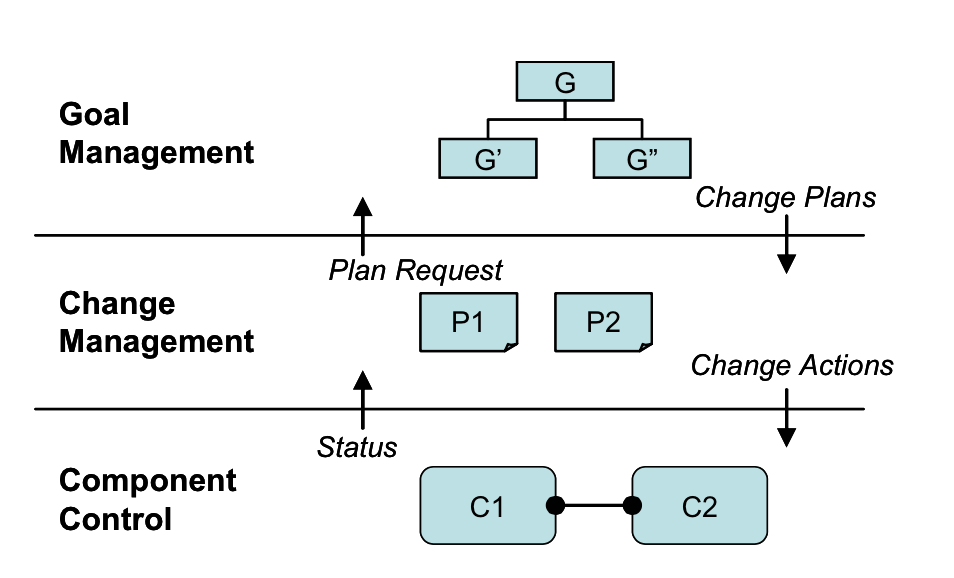
\includegraphics[width=\columnwidth]{three_layered_architecture}
	\caption{Three Layer Architecture Model for Self-Management \citep{Kramer:2007ff}}
	\label{fig:ch03_three_layer_architecture}
\end{figure}

\subsubsection{Reflection Reference Model}
\cite{Andersson:2009bq} propose a reference model for reflection (see Figure \ref{fig:ch03_reflection_reference_model}). The model consists of two parts, the \emph{meta-level} and the \emph{base-level}. The \emph{base-level} provides the functionality of the system and contains a computation part and a domain model. The \emph{meta-level} provides the reflective capability and consists of two parts, \emph{meta-computation} and \emph{meta-model}. The \emph{meta model} is the self-representation of the system. \emph{Meta-computation} is the logic dealing with the changes in the \emph{meta model}.

\begin{figure}[htbp]
	\centering
	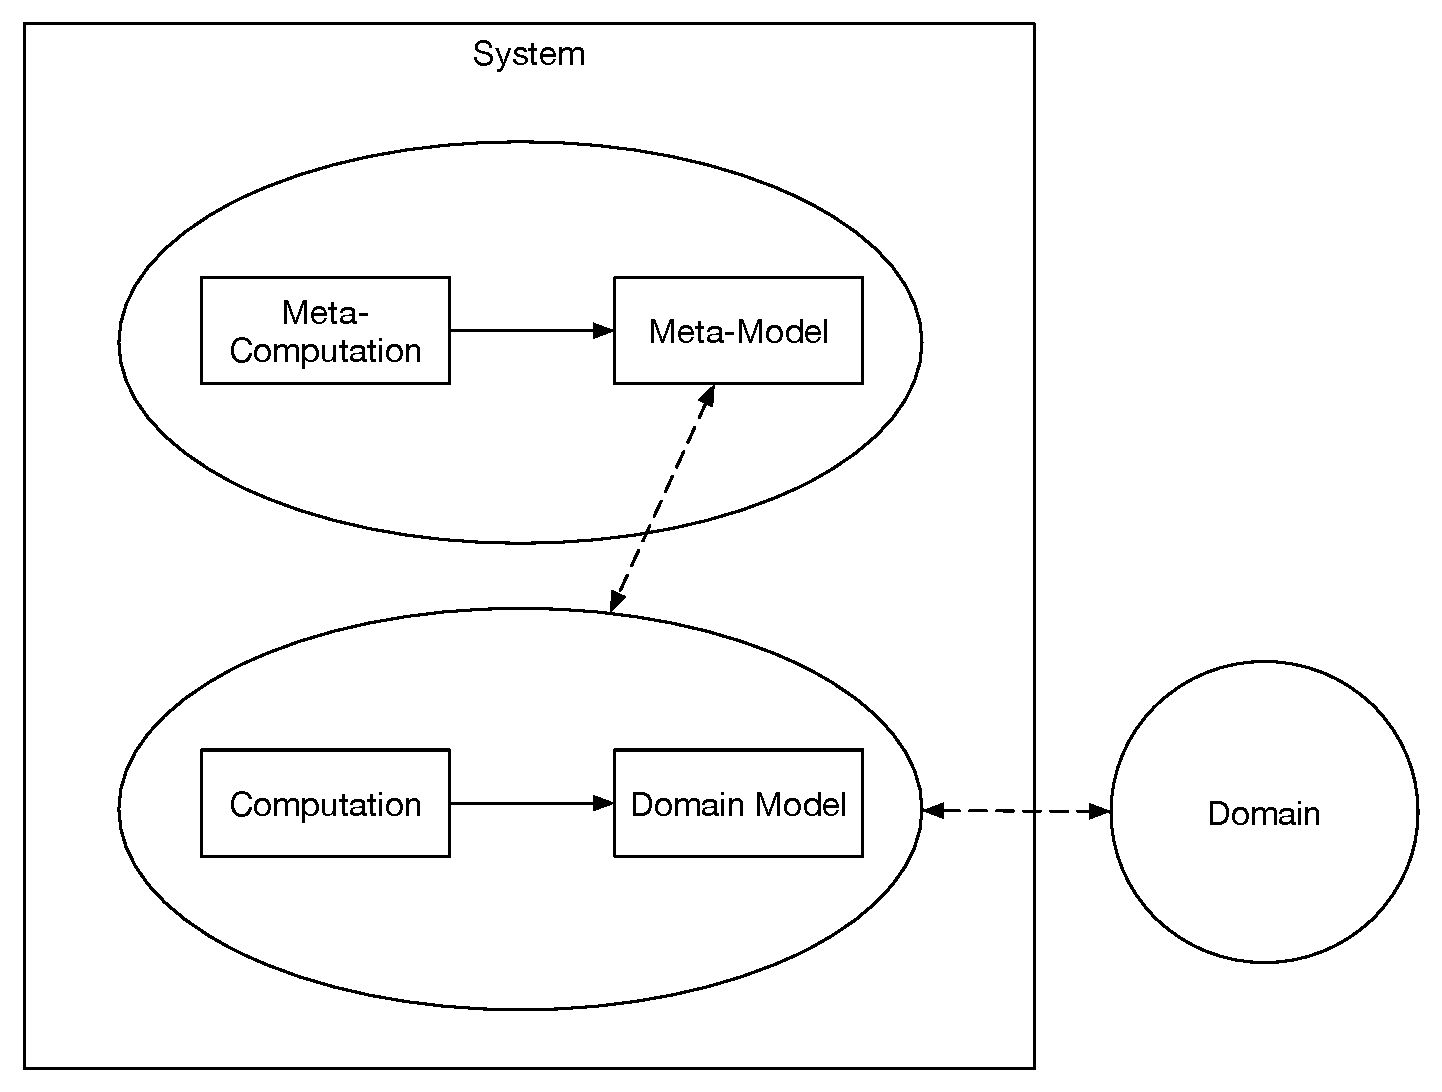
\includegraphics[width=\columnwidth]{ch3_reflection_reference_model}
	\caption{Reflection Reference Model \citep{Andersson:2009bq}}
	\label{fig:ch03_reflection_reference_model}
\end{figure}

\subsubsection{Mape-K}
IBM's \emph{Mape-K} (\emph{Monitor - Analyze - Plan - Execute - Knowlegde}) describes a reference architecture for adaptation control loops \citep{Group:2005ug}. It consists of the following elements:
\begin{itemize}
	\item \textbf{Monitor}\\
	The monitor function collects the details from the managed resources, via touchpoints, and correlates them into symptoms that can be analyzed.
	\item \textbf{Analyze}\\
	The analyze function provides the mechanisms to observe and analyze situations to determine if some change needs to be made.
	\item \textbf{Plan}\\
	The plan function creates or selects a procedure to enact a desired alteration in the managed resource.
	\item \textbf{Execute}\\
	The execute function provides the mechanism to schedule and perform the necessary changes to the system.
	\item \textbf{Knowledge}\\
	The four functions (monitor, analyze, plan, execute) share data in the \emph{Knowledge Source}, which includes topology information, historical logs, metrics, symptoms and policies.
\end{itemize}

\begin{figure}[htbp]
	\centering
	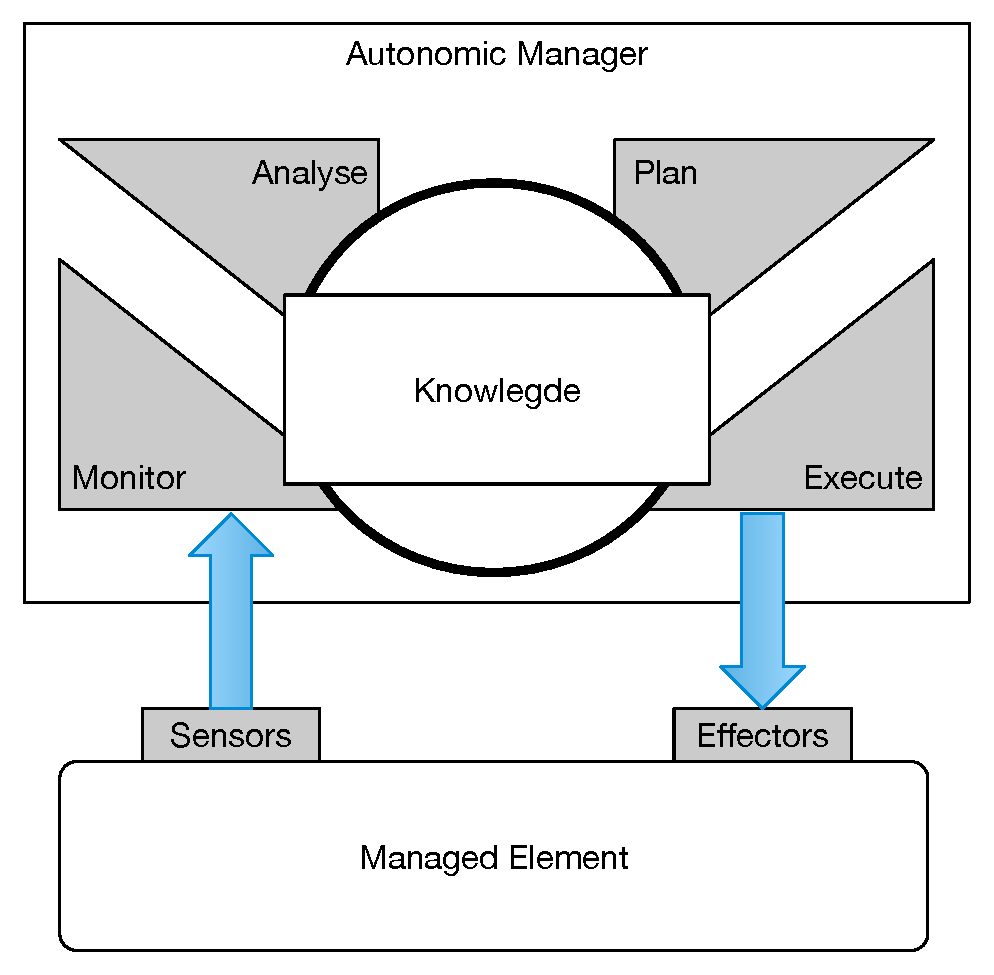
\includegraphics[width=0.8\columnwidth]{mape_k}
	\caption{Mape-K Reference Model \citep{Group:2005ug}}
	\label{fig:ch03_mape_k}
\end{figure}

\section{Self-Adaptive Middleware}

\citet{Duran-Limon:2004mi} argue that ``the most adequate level and natural locus for applying adaption is at the middleware level''. Adaption at the operating system level is platform-dependent and changes at this level affect every application running on the same node. On the other hand, adaption at application level assigns the responsibility to the developer and is also not reusable.

\citet{Lee:2009vn} propose an adaptive, general-purpose runtime infrastructure for effective resource management of the infrastructure. Their approach is comprised of three components:
\begin{enumerate}
	\item dynamic performance prediction
	\item adaptive intra-site performance management
	\item adaptive inter-site resource management
\end{enumerate}

The runtime infrastructure is able to choose from a set of performance predictions for a given service and to dynamically choose the most appropriate prediction over time by using the prediction history of the service.

AutoGlobe \citep{Gmach:2008vo} provides a platform for adaptive resource management comprised of 
\begin{enumerate}
	\item Static resource management
	\item Dynamic resource management
	\item Adaptive control of Service Level Agreements (SLA)
\end{enumerate}
Static resource management optimizes the allocation of services to computing resources and is based on on automatically detected service utilisation patterns. Dynamic resource management uses a fuzzy controller to handle exceptional situations at runtime. The Adaptive control of \acp{SLA} schedules service requests depending on their \ac{SLA} agreement.

The coBRA framework proposed by \citet{Irmert:2008nx} is an approach to replace service implementations at runtime as a foundation for self-adaptive applications. The framework facilitates the replacement of software components to switch the implementation of a service with the interface of the service staying the same.

DREAM (Dynamic Reflective Asynchronous Middleware) \citep{Leclercq:2004ly} is a component-based framework for the construction of reflective Message-Oriented Middleware. Reflective middleware ``refers to the use of a causally connected self-presentation to support the inspection and adaption of the middleware system'' \citep{Kon:2002fu}. DREAM is based on FRACTAL, a generic component framework and supports various asynchronous communication paradigms such as message passing, event-reaction and publish/subscribe. It facilitates the construction and configuration of Message-Oriented Middleware from a library of components such as message queues, filters, routers and aggregators, which can be assembled either at deploy-time or runtime.

\subsection{Adaption in Service-Oriented Architectures}
Several adaption methods have been proposed in the context of service-based applications. In their survey, \cite{Kazhamiakin:2010ub} describe the following adaption methods:
\begin{itemize}
	\item \textbf{Adaption by Dynamic Service Binding}\\
	This adaption method relies on the ability to select and dynamically substitute services at run-time or at deployment-time. Services are selected in such a way that the adaption requirements are satisfied in the best possible way. 
	\item \textbf{\ac{QoS}-Driven Adaption of Service Compositions}\\
	The goal of this adaption approach is to select the best set of services available at run-time, under consideration of process constraints, end-user preferences and the execution context.
	\item \textbf{Adaption of Service Interfaces and Protocols}\\
	The goal of this adaption approach is to mediate between two services with different signatures, interfaces and protocols. This includes signature-based adaption, ontology-based adaption or behavior-based adaption.
\end{itemize}

\subsection{Adaptive ESB}

Research on messaging middleware currently focusses on \ac{ESB} infrastructure. An \ac{ESB} is an integration platform that combines messaging, web services, data transformation and intelligent routing to connect multiple heterogeneous services \citep{Chappell:2004jo}. It is a common middleware to implement the integration layer of an Service Oriented Architecture (SOA) and is available in numerous commercial and open-source packages.

Several research has been done to extend the static service composition and routing features of standard ESB implementations with dynamic capabilities decided at run-time, such as dynamic service composition \citep{Chang:2007aa}, routing \citep{Bai:2007aa} \citep{Wu:2008aa} \citep{Ziyaeva:2008aa} and load balancing \citep{Jongtaveesataporn:2010aa}.

The DRESR (Dynamic Reconfigurable ESB Service Routing), proposed by \cite{Bai:2007aa}, allows the routing table to be changed dynamically at run-time based on service selection preferences, such as response time. It defines mechanisms to test and evaluate the availability and performance of a service and to select services based on its testing results and historical data.

\cite{Ziyaeva:2008aa} propose a framework for content-based intelligent routing. It evaluates the service availability and selects services based on its content and properties.

\cite{Jongtaveesataporn:2010aa} propose a load balancing me\-chanism that distributes requests to services of the same \emph{service type}, having the same function and signature, and enables the dynamic selection of the target service.

Work to manage and improve the \ac{QoS} of \ac{ESB} and service-based systems in general is mainly focussed on dynamic service composition and service selection based on monitored QoS metrics such as throughput, availability and response time \citep{Calinescu:2011aa}. 

\cite{Gonzalez:2011} propose an adaptive \ac{ESB} infrastructure to adress \ac{QoS} issues in service-based systems which provides adaption strategies for response time degradation and service saturation, such as invoking an equivalent service, using previously stored information, distributing requests to equivalent services, load balancing and deferring service requests.

In contrast to this solutions, the approach presented in this thesis uses dynamic message aggregation and message routing as adaption mechanism to optimize the end-to-end latency of messaging system for different load scenarios.

\section{Feedback Control of Computing Systems}

Control Engineering Methodologies have been identified as a promising solution to implement self-adaptive software systems \citep{Patikirikorala:2012ky}, especially for performance control \citep{Abdelzaher:2003ea}. In particular, feedback loops provide generic mechanisms for self-adaption \citep{Brun:2009ww}.  Control engineering is based on control theory, which provides a systematic approach to designing closed loop systems that are stable, accurate, have short settling times, and do not overshoot \citep{Abdelzaher:2008ub}.

The purpose of a controller is called control objective, the most common control objectives are \citep{Abdelzaher:2008ub}:
\begin{itemize}
	\item \textbf{Regulatory control}\\
	Ensure that the measured output is equal to (or near) the reference input.
	\item \textbf{Disturbance rejection}\\
	Ensure that disturbances acting on the system do not significantly affect the measured output.
	\item \textbf{Optimization}\\
	Obtain the best value of the measured output.
\end{itemize}

\begin{figure}[htbp]
	\centering
	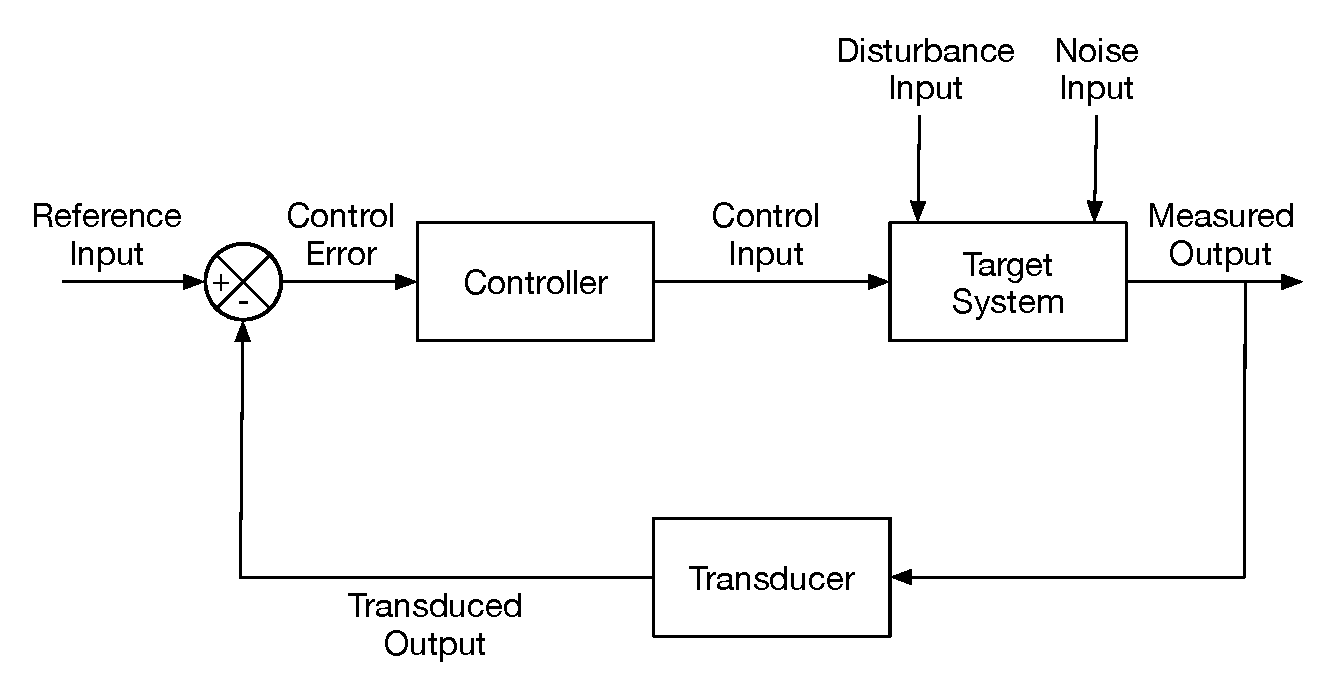
\includegraphics[width=\columnwidth]{ch3_feedback_control_system}
	\caption{Block diagram of feedback control system \citep{Hellerstein:2004a}}
	\label{fig:ch03_feedback_control_system}
\end{figure}

Figure \ref{fig:ch03_feedback_control_system} shows the essential elements of a single-input, single-output (SISO) control system \citep{Hellerstein:2004a}:
\begin{itemize}
	\item \textbf{Control error}\\
	The difference between the reference input and the measured output.
	\item \textbf{Control input}\\
	The parameter that affects the behaviour of the controlled system.
	\item \textbf{Controller}\\
	The controller determines the setting of the control input needed to achieve the reference input.
	\item \textbf{Disturbance input}\\
	Any change that affects the way in which the control input influences the measured output.
	\item \textbf{Measured output}\\
	The measurable parameter of the controlled system.
	\item \textbf{Noise input}\\
	Any effect that changes the measured output produced by the controlled system.
	\item \textbf{Reference Input}\\
	The desired value of the measured output.
	\item \textbf{Target system}\\
	The computing system to be controlled.
\end{itemize}

Feedback-control has been applied to several different domains of computing systems since the early 1990s, including data networks, operating systems, middleware, multimedia and power management (cf. \cite{Hellerstein:2004a}). Feedback-control of middleware systems include application servers, such as the Apache http-Server, database management systems, such as IBM Universal Database Server, and e-mail servers, such as the IBM Lotus Domino Server. \cite{Hellerstein:2004a} describe 3 basic control problems in this context:
\begin{itemize}
	\item Enforcing service level agreements
	\item Regulate resource utilization
	\item Optimize the system configuration
\end{itemize}

Additionally, feedback-control has been applied recently to web environments, such as web servers and web services, application servers, including data flow control in J2EE servers, Repair Management in J2EE servers and improving the performance of J2EE servers and cloud environments (cf. \cite{Gullapalli:2011vn}).

According to \cite{Patikirikorala:2012ky}, approaches for feedback-control of computing systems use the following control mechanisms:
\begin{itemize}
	\item \textbf{Fixed-gain control}\\
	Fixed-gain control uses static model parameters and gains, for example \ac{PID}-controllers.
	\item \textbf{Adaptive control}\\
	Adaptive control dynamically estimates the model parameters and gains of the controller at runtime.
	\item \textbf{Linear Quadratic Regulator (LQR)}\\
	LQR is an optimal control strategy particular useful in the MIMO control systems design. It uses a cost function representing a quadratic formula involving the control error and control effort. The goal is to mimimize the cost function so that the error is minimized with a small control effort.
	\item \textbf{Model predictive control (MPC)}\\
	MPC control algorithms aim to optimize the future behavior by computing the trajectory of the control inputs. 
	\item \textbf{Gain scheduling}\\
	Gain scheduling uses a predefined logic/rule based evaluation to change the controller online. These rules are implemented in the gain scheduling component and depend on the prior knowledge about the performance variables, disturbances and conditions.
	\item \textbf{Cascaded (nested) control}\\
	The objective of cascaded control is to change the set point of the inner loop by an outer loop.
\end{itemize}

A fixed-gain controller that is widely used in exisiting approaches is a \ac{PID}-Controller because of its robustness against modelling errors, disturbance rejection capabilities and simplicity (cf. \cite{Patikirikorala:2012ky}). It calculates the output value $u_k$ at time step $k$ of the controller depending on the current (proportional part), previous (integral part) and expected future error (differential part):
\begin{displaymath}
	u_k=K_p*e_k+K_i*T_a\sum_{i=0}^k e_i+\frac{K_d}{T_a}(e_k-e_{k-1})
\end{displaymath}
with $K_p$ being the controller gain of the proportional part, $e_k$ being the error ($r-y$) at step $k$, $K_i$ being the controller gain of the integral part, $T_a$ being the sampling interval and $K_d$ being the controller gain of the differential part.

The \emph{Adaptive Middleware} presented in this thesis utilizes a closed-feedback loop to control the aggregation size of the processed messages, depending on the current load of the system to minimize the end-to-end latency of the system. This is a novel approach that has not previously been investigated.

\section{SLA-Monitoring of Business Processes}
The SECMOL framework (Service Centric Monitoring Language), developed by \citet{Guinea:2009fk}, allows to monitor the quality of service constraints of BPEL processes. It is comprised of three components. Data Collectors for capturing data, Data Analyzers for analysing the captured data and the Monitoring Manager for coordinating the monitoring process. SECMOL also defines a XML-based monitoring specification, which consists of monitoring policies that specify how the monitoring should be done and monitoring rules that express the quality of service properties the system needs to satisfy.

\citet{Duc:2009kx} argue that a monitoring middleware component should fulfill the following requirements:
\begin{itemize}
	\item \textbf{Coherency of data}\\
	All data used in one decision must reflect the same state of the system.
	\item \textbf{Flexibility in data access}\\
	Every monitored service provider should be able to respond using its own measurement units. This should be transparent for the client using the monitoring data.
	\item \textbf{Performance in data access}\\
	The monitoring should have the slightest possible impact on the performance of the business process.
	\item \textbf{Network usage optimisation}\\
	The transmission of monitoring data should have the slightest possible impact on the network performance.
\end{itemize}
The authors propose M4ABP (Monitoring for Adaptive Business Process), a distributed monitoring and data delivery middleware subsystem which implements these requirements.

SALMon \citep{Ameller:2008zr} is a system for monitoring the services of an \ac{SOA} for \acf{SLA} violations. It is itself implemented as a service-oriented system and consists of the following services:
\begin{itemize}
	\item \textbf{Monitor}\\
	The Monitor service collects the monitoring data from components called Measure Instruments that are instantiated in each monitored service. 
	\item \textbf{Analyzer}\\
	The Analyzer service manages the Monitor service and checks for Service Level Agreement violations of the monitored services.
	\item \textbf{Decision Maker}\\
	The Decision Maker service is able to select an action to solve the SLA violation. The appropriate action for a specific SLA violation is stored in a repository.
\end{itemize}
The attributes measured by SALMon are taken from an ISO/IEC 9126-1-based quality model.

\citet{Textor:2009vn} propose an approach to map implementation level monitoring data to business level activities. Non-functional constraints are specified on a workflow model in the modelling phase. Additionally, an instrumentation model is used to specify the instrumentation points of the application. At runtime, the monitoring data of the system is mapped to the workflow model. 
The monitoring data is received by a component called ConstraintMonitor, which evaluates and validates the constraints specified in the workflow model.

\citet{Wetzstein:2009uq} present a framework to monitor and analyse the factors that influence the performance of WS-BPEL processes. The authors distinguish between PPM (Process Performance Metrics) and QoS (Quality of Service) metrics, which influence the Key Performance Indicators (KPI) of business processes. PPMs are based on process runtime events, that are published by the WS-BPEL runtime engine, for example the ``number of orders which can be served as inhouse stock''. QoS metrics are technical parameters of the underlying services that implement the business process, for example the response time and availability of a service. KPIs are based on business goals, for example ``order fulfillment lead time < 3''. The proposed framework monitors KPIs, PPMs and QoS metrics at runtime, which are modeled in a Process Metrics Definition Model (PMDM). These collected metrics can then be used to perform a dependency analysis of the influential factors of a KPI using machine learning techniques to construct dependency trees.

iBOM \citep{Castellanos:2005fk} is a platform to analyze, manage and optimize business operations based on business goals. Optimizations are performed by using simulation techniques. iBom simulates different configurations of a business process to identify the configuration that best meets the business goals. First, the user needs to define the optimization metric and constraints on this metric and on the resources. The configuration candidates are then either computed by iBOM using different resource allocations of the given configuration within the defined constraints or are provided by the user in the form of a process model. 

\section{Summary}

Most of the work done in the field of performance of service-oriented systems involves performance aspects of Web Services including the SOAP standard. This includes performance modeling, performance measuring and performance optimisation.

Approaches to optimize the transfer of bulk data of Web services, as proposed by \citet{Wichaiwong:2007oq} and  \citet{Habich:2007ij} deliver an overall better performance than using SOAP. However, like a traditional batch-processing system using file- or database-based integration, they are not able to reduce the latency and thus cannot deliver near-time processing of bulk data.

Current self-adapting middleware platforms, like the AutoGlobe platform \citep{Gmach:2008vo}, are focused on adaptive resource management to dynamically allocate services to computing nodes or to replace service implementations at runtime, as proposed by the coBRA framework \citep{Irmert:2008nx}.

Several research has been done to extend the static service composition and routing features of standard ESB implementations with dynamic capabilities decided at run-time, such as dynamic service composition \citep{Chang:2007aa}, routing \citep{Bai:2007aa} \citep{Wu:2008aa} \citep{Ziyaeva:2008aa} and load balancing \citep{Jongtaveesataporn:2010aa}.

Feedback-control is a common technique to implement the adaptive behaviour of software systems. In this thesis, a closed feedback-loop is used to control aggregation size of messaging system to minimize the end-to-end latency of the system.

Work on SLA-monitoring of business processes proposes different approaches to monitor the compliance of a business process to Service Level Agreements, which include the end-to-end latency and throughput of the business process. 

This thesis proposes an adaptive middleware to optimize the end-to-end latency of a system for bulk data processing by dynamically adapting its processing style between batch and single-event processing, based on the current load of the system. This is a novel approach which has not yet been discussed in current literature.

While the research presented in this thesis is based on previous work in the fields of self-adaptive middleware and feeback-control of computing systems, 
the work discussed in this chapter does not offer a solution for the research question stated in Section \ref{sec:research_objectives}: How to achieve high-performance near-time processing of bulk data?